\documentclass{standalone}
\usepackage{tikz}
\usepackage{textcomp}

\begin{document}

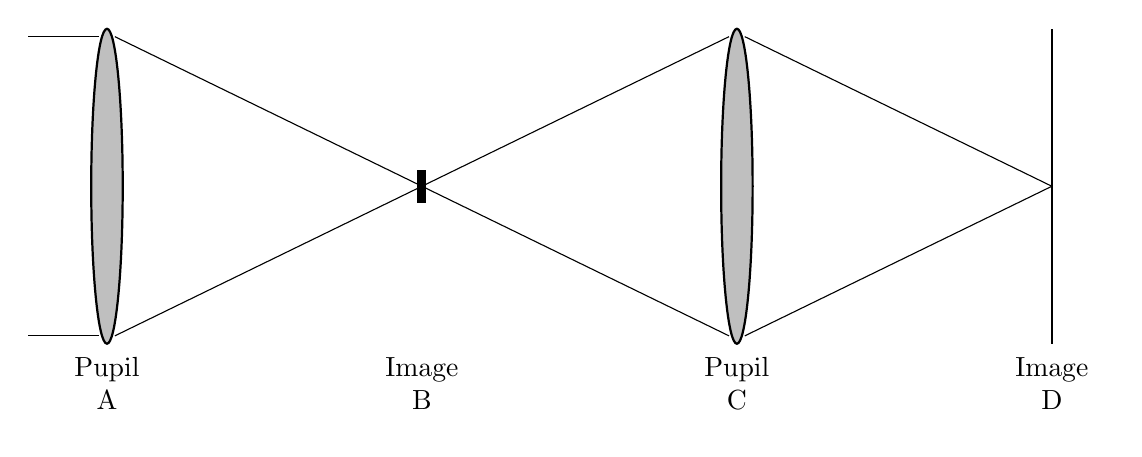
\begin{tikzpicture}

    \draw[thick, fill=lightgray] (0,0) circle [x radius=0.2, y radius=2];
    \node[below] at (0,-2) {\begin{tabular}{c}Pupil\\A\end{tabular}};

    \node[below] at (4,-2) {\begin{tabular}{c}Image\\B\end{tabular}};
    \draw[fill=black] (3.95,0.2) rectangle (4.05,-0.2);
     
    \draw[thick, fill=lightgray] (8,0) circle [x radius=0.2, y radius=2];
    \node[below] at (8,-2) {\begin{tabular}{c}Pupil\\C\end{tabular}};

    \draw[thick] (12,-2) -- (12,2);
    \node[below] at (12,-2) {\begin{tabular}{c}Image\\D\end{tabular}};

    \draw (-1,1.9) -- (-0.1,1.9);
    \draw (0.1,1.9) -- (7.9,-1.9);
    \draw (8.1,1.9) -- (12,0);

    \draw (-1,-1.9) -- (-0.1,-1.9);
    \draw (0.1,-1.9) -- (7.9,1.9);
    \draw (8.1,-1.9) -- (12,0);

\end{tikzpicture}
\end{document}
